\documentclass[11pt]{article}
\usepackage[T1]{fontenc}
\usepackage{lmodern}
\usepackage{amsmath,amssymb,amsthm,mathtools}
\usepackage[letterpaper,margin=1in]{geometry}
\usepackage{microtype}
\usepackage{enumitem}
\usepackage{booktabs}
\usepackage{graphicx}
\usepackage{tikz}
\usetikzlibrary{arrows.meta,calc,positioning}
\usepackage{xcolor}
\definecolor{linkblue}{HTML}{23527C}
\definecolor{parentblue}{HTML}{28698D}
\definecolor{childorange}{HTML}{B76223}
\usepackage[colorlinks=true,linkcolor=linkblue,citecolor=linkblue,urlcolor=linkblue]{hyperref}
\usepackage[capitalise,noabbrev]{cleveref}
\hypersetup{pdftitle={Thompson's group F is nonamenable}}

\newcommand{\unverified}[1]{\par\smallskip\noindent\fbox{\parbox{0.95\linewidth}{\textbf{Unverified step.} #1}}\par\smallskip}

\newcommand{\R}{\mathbb R}
\newcommand{\N}{\mathbb N}
\newcommand{\Z}{\mathbb Z}
\newcommand{\norm}[1]{\lVert #1\rVert}
\newcommand{\ip}[2]{\langle #1,#2\rangle}
\newcommand{\id}{\mathrm{id}}
\newcommand{\cI}{\mathcal I}
\newcommand{\EA}{\mathbb E_A}
\DeclareMathOperator{\Lip}{Lip}
\DeclareMathOperator{\dist}{dist}
\DeclareMathOperator{\sinc}{sinc}
\newtheorem{theorem}{Theorem}[section]
\newtheorem{lemma}[theorem]{Lemma}
\newtheorem{proposition}[theorem]{Proposition}
\newtheorem{corollary}[theorem]{Corollary}
\theoremstyle{definition}
\newtheorem{definition}[theorem]{Definition}
\newtheorem{remark}[theorem]{Remark}
\newtheorem{example}[theorem]{Example}
\numberwithin{equation}{section}
\setlist[itemize]{topsep=4pt,itemsep=2pt,parsep=0pt}
\setlist[enumerate]{topsep=4pt,itemsep=2pt,parsep=0pt}
\setlength{\emergencystretch}{2em}

\title{Thompson's group \(F\) is nonamenable}
\author{Rewritten for readability from the OpenAI manuscript of the same title}
\date{September 23, 2026}

\begin{document}
\maketitle
\begin{abstract}
The source manuscript proves that Thompson's group \(F\) is nonamenable,
confirming Geoghegan's conjecture. This rewrite presents the same proof,
with the same statements and constants, as a sequence of individually
checkable steps. One step in the proof of an auxiliary lemma
(Lemma~\ref{dyad:transport}) is flagged: as worded in the source it does
not justify the next sentence, although the lemma itself is not in doubt.
\end{abstract}

\section{The result and the plan}
\label{sec:introduction}

\subsection{Statement}

\emph{Thompson's group} \(F\) consists of the increasing piecewise linear
homeomorphisms of \([0,1]\) with finitely many linear pieces, dyadic
rational breakpoints, and slopes in \(2^{\Z}\). The group law is
composition, \(hg=h\circ g\), and \(F\) is regarded as a discrete group.

A discrete group \(\Gamma\) is \emph{amenable} if there is a linear
functional \(\mu:\ell^\infty(\Gamma;\R)\to\R\) with \(\mu(1)=1\),
\(\mu(\psi)\ge0\) whenever \(\psi\ge0\), and
\(\mu(g\mapsto\psi(hg))=\mu(\psi)\) for every \(h\in\Gamma\)
(a positive normalized left-invariant mean). This viewpoint belongs to the
classical theory of von Neumann and Day \cite{vonNeumann1929,Day1957}.

The proof uses amenability only through one cited fact, the forward
implication of the F\o lner criterion \cite{Folner1955}:

\begin{quote}
\emph{If \(\Gamma\) is amenable, then for every finite \(S\subset\Gamma\)
and every \(\varepsilon>0\) there is a nonempty finite \(A\subset\Gamma\)
such that}
\begin{equation}\label{eq:folner}
  \frac{|hA\mathbin{\triangle}A|}{|A|}<\varepsilon
  \qquad(h\in S).
\end{equation}
\end{quote}
Here \(hA=\{hg:g\in A\}\) and \(\triangle\) is symmetric difference. The
source adds that the left-translation formulation in
\cite[Theorem~1.2]{Moore2013} bounds the sum of these ratios over
\(h\in S\), which implies each individual bound.

Thompson introduced \(F\) in 1965; an early published construction appears
in McKenzie and Thompson \cite{McKenzieThompson1973}, with the
identification explained by Cannon, Floyd, and Parry
\cite[pp.~215--216]{CannonFloydParry1996}, who also record Geoghegan's 1979
conjecture that \(F\) is nonamenable \cite[p.~227]{CannonFloydParry1996}.

\begin{theorem}[source Theorem~1.1]\label{thm:main}
Thompson's group \(F\) is not amenable.
\end{theorem}

By \eqref{eq:folner}, it suffices to exhibit \emph{one} finite set
\(S\subset F\) and \emph{one} constant \(c_0>0\) such that every nonempty
finite \(A\subset F\) satisfies
\(\max_{h\in S}|hA\triangle A|/|A|\ge c_0\). This is
Proposition~\ref{avg:boundary}.

\subsection{The one external ingredient}

\begin{lemma}[Benyamini--Sternfeld; source Lemma~1.2]\label{lem:displacement}
There are a real Hilbert space \(H\), a Lipschitz map \(f:B\to B\) on its
closed unit ball \(B\), and a constant \(\delta>0\) such that
\[
  \norm{f(x)-x}\ge\delta\qquad(x\in B).
\]
\end{lemma}

\noindent\emph{Justification.} Two are offered. (i) The source cites
\cite[Theorem, part~(3), p.~439]{BenyaminiSternfeld1983}, which it says
proves this assertion for every infinite-dimensional normed space.
(ii) Appendix~\ref{app:auxiliary} constructs such a map on
\(H=L^2([0,1];\R^2)\) with \(\delta=1/2\)
(Proposition~\ref{aux:map}). The appendix uses nothing from
Sections~\ref{sec:dyadic}--\ref{sec:boundary}. In finite dimensions the
lemma is false by Brouwer's theorem, so infinite dimensionality is
essential.

\subsection{Proof at a glance}\label{sec:glance}

\paragraph{Key idea.}
Fix \(f,\delta\) from Lemma~\ref{lem:displacement}, a Lipschitz constant
\(L\) of \(f\), and a large integer \(D\). Choose \(D\) disjoint dyadic
intervals \(I_1<\dots<I_D\) in \((0,1)\) (``parents'') and, inside each
parent \(I_i\), the affine copies \(I_i\cdot I_j\) of the same family
(``children''). To every finite dyadic partition \(T\) of \([0,1]\) one
attaches a vector \(p(T)\in B\) (its ``color'') by the recursion
\[
  p(T)=f\Bigl(\tfrac1D\textstyle\sum_{j}p(T_{I_j})\Bigr),
\]
where \(T_{I_j}\) is the part of \(T\) inside \(I_j\), rescaled to
\([0,1]\). For \(g\in F\) and a fine level \(n\), let \(X_I(g)\) be the
color of the image partition \(gT^{(n)}\) seen through the interval \(I\).
Two exact facts drive the proof.
\begin{itemize}
\item \emph{Recursion.} \(X_{I_i}(g)=f(z_i(g))\), where \(z_i(g)\) is the
mean of the \(D\) child colors \(X_{I_i\cdot I_j}(g)\).
\item \emph{Covariance.} If \(h\in F\) carries intervals \(I<J\) affinely
onto \(I_1<I_2\), then \(X_I(g)=X_{I_1}(hg)\) and \(X_J(g)=X_{I_2}(hg)\).
\end{itemize}
Let \(S\) be a finite set containing one such \(h\) for each separated
pair \(I<J\) of parents and children, and let \(A\subset F\) be finite
with all ratios \(|hA\triangle A|/|A|\le\eta\) for \(h\in S\). Covariance
then forces the \(A\)-averages of \(\ip{X_I}{X_J}\) to agree, up to
\(\eta\), with a single number \(\alpha\), for \emph{all} separated pairs.
Let \(m(g)\) be the mean of the parent colors. Expanding
\(\norm{z_i-m}^2\) into inner products, all but a fraction \(1/D\) of the
terms are separated pairs, and the \(\alpha\)'s cancel:
\[
  \EA\norm{z_i-m}^2\le \tfrac4D+4\bigl(1-\tfrac1D\bigr)\eta .
\]
But \(m\) is the mean of the \(f(z_i)\), so \(z_i\approx m\) for all \(i\)
forces \(m\approx f(m)\), which Lemma~\ref{lem:displacement} forbids.
Quantitatively, \(\delta^2\le L^2\bigl(4/D+4(1-1/D)\eta\bigr)\), so \(\eta\)
is bounded below once \(D>4L^2/\delta^2\).

\paragraph{Steps and dependencies.}
\begin{itemize}
\item Lemma~\ref{dyad:calculus} (restriction calculus,
\((T_I)_J=T_{I\cdot J}\)) \(\to\) Lemma~\ref{color:welldefined}
(the coloring is well defined) and Step~2 of
Proposition~\ref{avg:boundary} (recursion identity).
\item Lemma~\ref{dyad:nested} \(\to\) Lemma~\ref{dyad:eventual}
(\(gT^{(n)}\) is eventually basic and fine) \(\to\) choice of the level
\(n\) in Step~0 of Proposition~\ref{avg:boundary}.
\item Lemma~\ref{dyad:transport} (transport of pairs of intervals)
\(\to\) definition of the finite set \(S\) (Section~\ref{sec:boundary}).
\item Lemma~\ref{dyad:covariance} (covariance) \(+\)
Lemma~\ref{lem:finite-translation} (finite averages under translation)
\(\to\) Step~1 of Proposition~\ref{avg:boundary} (all separated
correlations are within \(\eta\) of \(\alpha\)).
\item Lemma~\ref{lem:displacement} \(\to\) definition of the coloring and
Step~3 (pointwise displacement inequality).
\item Steps~1--5 \(\to\) Proposition~\ref{avg:boundary} \(\to\)
Theorem~\ref{thm:main}, via \eqref{eq:folner}.
\end{itemize}
Section~\ref{sec:consequences} records two corollaries that quote
companion papers; they are not used in the proof.

\subsection{Context and prior work (not used in the proof)}
The source records the following background. Brin and Squier show that
\(F\) contains no nonabelian free subgroup
\cite[Theorem~3.1]{BrinSquier1985}, so the free-subgroup obstruction to
amenability does not apply. Yet \(F\) is not elementary amenable
\cite[Theorem~4.10]{CannonFloydParry1996}. Brown and Geoghegan construct a
classifying space for \(F\) with finitely many cells in each dimension
\cite{BrownGeoghegan1984}. Moore proves tower lower bounds on the sizes of
possible F\o lner sets \cite[Theorem~1.1]{MooreFolner2013} and
characterizes amenability of \(F\) by a scalar convex Ramsey property for
finite rooted ordered binary trees \cite[Theorem~3.1]{Moore2013}. Guba
improves densities of finite Cayley subgraphs \cite{Guba2025Density} and
derives restrictions on right-invariant means from a partition into seven
diagram-defined classes \cite{Guba2026}. Haagerup and Olesen prove that
simplicity of the reduced group \(C^*\)-algebra of Thompson's group \(T\)
would imply nonamenability of \(F\)
\cite[Theorem~5.5]{HaagerupOlesen2017}. There have also been claims of a
complete resolution in both directions: Akhmedov's 2021 version claims
nonamenability through a height-function criterion \cite{Akhmedov2021};
Shavgulidze claimed amenability \cite{Shavgulidze2009}, and Moore
identified errors in that approach \cite{Moore2011Critique}; Moore
separately withdrew an amenability claim after Akhmedov identified an
error in Lemma~4.13 of that manuscript \cite{Moore2012Withdrawn}, a
different work from his published Ramsey characterization.

\subsection{Conventions and changes of notation}
The mathematics is that of the source. To keep each symbol to one meaning,
a few letters were changed: the generic group is \(\Gamma\) and the mean
is \(\mu\) (source: \(G\), \(M\)); the finite set of group elements in
Lemma~\ref{dyad:eventual} is \(E\) (source: \(K\)); cells of partitions
are always \(C\); in Section~\ref{sec:consequences} and in the appendix
some letters are renamed as stated there. The inline facts of the source's
Section~2.1 are stated here as Lemmas~\ref{dyad:calculus},
\ref{dyad:nested} and~\ref{dyad:covariance}; source numbers are given in
the headings of the other results.

\section{Dyadic partitions and affine transport}\label{sec:dyadic}

The source uses the standard dyadic-partition model of \(F\) and points to
\cite[Section~2, Lemma~2.2]{CannonFloydParry1996}; everything needed is
proved below.

\begin{definition}\label{dyad:defs}
\begin{enumerate}[label=(\alph*)]
\item A \emph{basic dyadic interval} (of level \(\ell\)) is an interval
\([k2^{-\ell},(k+1)2^{-\ell}]\subseteq[0,1]\) with
\(\ell\in\N\cup\{0\}\) and \(0\le k<2^\ell\).
\item A \emph{basic partition} is a finite set \(T\) of basic intervals
(its \emph{cells}) that cover \([0,1]\) and have pairwise disjoint
interiors. Its \emph{mesh} is the greatest length of a cell. \(T\)
\emph{respects} an interval \(I\) if \(I\) is a union of cells of \(T\).
\item For a basic interval \(I\), \(s_I:[0,1]\to I\) is the increasing
affine bijection, and \(I\cdot J=s_I(J)\) for a basic interval \(J\).
If \(T\) respects \(I\), its \emph{normalized restriction} is
\[
  T_I=\{s_I^{-1}(C):C\in T,\ C\subseteq I\}.
\]
\item \(T^{(n)}\) is the partition of \([0,1]\) into the \(2^n\) basic
intervals of level \(n\). For \(g\in F\), \(gT^{(n)}=\{g(C):C\in T^{(n)}\}\).
\item \(I<J\) means \(\max I<\min J\) (a positive gap is required). An
interval is \emph{internal} if both endpoints lie in \((0,1)\).
\end{enumerate}
\end{definition}

\begin{lemma}[restriction calculus]\label{dyad:calculus}
Let \(I=[k2^{-\ell},(k+1)2^{-\ell}]\) and \(J\) be basic intervals and
\(T\) a basic partition.
\begin{enumerate}[label=(\alph*)]
\item \(I\cdot J\) is a basic interval contained in \(I\), and
\(s_{I\cdot J}=s_I\circ s_J\).
\item If \(T\) respects \(I\), then \(T_I\) is a basic partition. It has
strictly fewer cells than \(T\) when \(I\ne[0,1]\).
\item If \(T\) respects both \(I\) and \(I\cdot J\), then \(T_I\) respects
\(J\) and
\begin{equation}\label{dyad:restriction}
  (T_I)_J=T_{I\cdot J}.
\end{equation}
\end{enumerate}
\end{lemma}
\noindent\emph{Used in:} Lemma~\ref{color:welldefined} (part (b)) and
Step~2 of Proposition~\ref{avg:boundary} (part (c)).

\begin{proof}
Note \(s_I(x)=2^{-\ell}(x+k)\) and \(s_I^{-1}(y)=2^{\ell}y-k\).

(a) If \(J=[j2^{-\ell'},(j+1)2^{-\ell'}]\), then
\(s_I(J)=[(k2^{\ell'}+j)2^{-(\ell+\ell')},(k2^{\ell'}+j+1)2^{-(\ell+\ell')}]\),
a basic interval of level \(\ell+\ell'\), contained in \(s_I([0,1])=I\).
Both \(s_{I\cdot J}\) and \(s_I\circ s_J\) are increasing affine
bijections \([0,1]\to I\cdot J\); such a map is unique.

(b) Let \(C\in T\) with \(C\subseteq I\). Then \(C\) has length
\(2^{-\ell'}\le 2^{-\ell}\), say \(C=[j2^{-\ell'},(j+1)2^{-\ell'}]\) with
\(\ell'\ge\ell\), and
\[
  s_I^{-1}(C)=\bigl[(j-k2^{\ell'-\ell})2^{-(\ell'-\ell)},\,
                    (j-k2^{\ell'-\ell}+1)2^{-(\ell'-\ell)}\bigr]
  \subseteq[0,1],
\]
an interval of length \(2^{-(\ell'-\ell)}\) whose left endpoint is an
integer multiple of that length: a basic interval. Since \(T\) respects
\(I\), the cells contained in \(I\) cover \(I\) with disjoint interiors;
applying the homeomorphism \(s_I^{-1}:I\to[0,1]\) gives a cover of
\([0,1]\) with disjoint interiors. So \(T_I\) is a basic partition.
The map \(C\mapsto s_I^{-1}(C)\) is a bijection from
\(\{C\in T:C\subseteq I\}\) onto \(T_I\). If \(I\ne[0,1]\), a point of
\([0,1]\setminus I\) lies in a cell of \(T\) not contained in \(I\), so
\(T_I\) has strictly fewer cells than \(T\).

(c) Since \(T\) respects \(I\cdot J\), we have
\(I\cdot J=\bigcup\{C\in T:C\subseteq I\cdot J\}\), and each such \(C\)
lies in \(I\) by (a). Applying \(s_I^{-1}\) gives
\(J=\bigcup\{s_I^{-1}(C)\}\), a union of cells of \(T_I\); so \(T_I\)
respects \(J\). Next, for \(C\in T\) with \(C\subseteq I\), we have
\(s_I^{-1}(C)\subseteq J\) iff \(C\subseteq s_I(J)=I\cdot J\). Hence, using
\(s_J^{-1}\circ s_I^{-1}=s_{I\cdot J}^{-1}\) from (a),
\[
  (T_I)_J=\{s_J^{-1}(s_I^{-1}(C)):C\in T,\ C\subseteq I\cdot J\}
         =\{s_{I\cdot J}^{-1}(C):C\in T,\ C\subseteq I\cdot J\}
         =T_{I\cdot J}.\qedhere
\]
\end{proof}

\begin{lemma}\label{dyad:nested}
\begin{enumerate}[label=(\alph*)]
\item Two basic intervals whose interiors intersect are nested.
\item A basic partition \(T\) whose mesh is smaller than the length of a
basic interval \(I\) respects \(I\).
\end{enumerate}
\end{lemma}
\noindent\emph{Used in:} Lemma~\ref{dyad:eventual}.

\begin{proof}
(a) Let \(I\) have level \(\ell\) and \(J\) level \(\ell'\ge\ell\). Every
multiple of \(2^{-\ell}\) is a multiple of \(2^{-\ell'}\), so the interior
of \(J\), which lies strictly between two consecutive multiples of
\(2^{-\ell'}\), contains no multiple of \(2^{-\ell}\). Hence \(J\) lies in
a single basic interval \(I'\) of level \(\ell\). If \(I'\ne I\), the
interiors of \(I\) and \(I'\) are disjoint, so those of \(I\) and \(J\)
are too. Thus if the interiors of \(I,J\) meet, then \(J\subseteq I\).

(b) Let \(x\) be an interior point of \(I\) and \(C\in T\) a cell
containing \(x\). As \(C\) is a nondegenerate interval through \(x\), its
interior meets the interior of \(I\). By (a) the two are nested, and
\(|C|<|I|\) gives \(C\subseteq I\). So the interior of \(I\) is contained
in \(\bigcup\{C\in T:C\subseteq I\}\subseteq I\). This finite union of
closed sets is closed, hence equals \(I\).
\end{proof}

\begin{lemma}[source Lemma~2.1]\label{dyad:eventual}
For each \(g\in F\), the partitions \(gT^{(n)}\) are basic for all
sufficiently large \(n\), and their meshes tend to zero. In particular,
given a finite set \(E\subset F\) and a finite family \(\mathcal J\) of
basic intervals, there is an \(n_0\) such that \(gT^{(n)}\) is basic and
respects every member of \(\mathcal J\) whenever \(g\in E\) and
\(n\ge n_0\).
\end{lemma}
\noindent\emph{Used in:} the choice of the level \(n\) in
Proposition~\ref{avg:boundary}.

\begin{proof}
\emph{Step 1 (normal form).} Let \(0=x_0<x_1<\dots<x_N=1\) be dyadic
points containing all breakpoints of \(g\), and let
\(g(x)=2^{q_i}x+b_i\) on \([x_{i-1},x_i]\), \(q_i\in\Z\). Each \(g(x_i)\)
is dyadic: \(g(x_0)=0\) and
\(g(x_i)=g(x_{i-1})+2^{q_i}(x_i-x_{i-1})\). Hence
\(b_i=g(x_{i-1})-2^{q_i}x_{i-1}\) is dyadic.

\emph{Step 2 (choice of \(n\)).} A dyadic rational is an integer multiple
of \(2^{-N'}\) for all large \(N'\). So there is \(n_g\) such that for all
\(n\ge n_g\): (i) every \(x_i\) is a multiple of \(2^{-n}\); (ii)
\(n\ge q_i\) for all \(i\); (iii) every \(b_i\) is an integer multiple of
\(2^{q_i-n}\).

\emph{Step 3 (cells map to basic intervals).} Let \(n\ge n_g\) and
\(C=[j2^{-n},(j+1)2^{-n}]\). By (i), \(C\) lies in one piece
\([x_{i-1},x_i]\), so
\(g(C)=[j2^{q_i-n}+b_i,(j+1)2^{q_i-n}+b_i]\subseteq[0,1]\). Its length is
\(2^{-(n-q_i)}\) with \(n-q_i\ge0\) by (ii), and its left endpoint is an
integer multiple of that length by (iii). So \(g(C)\) is basic. Since
\(g\) is a homeomorphism of \([0,1]\), the images of the cells of
\(T^{(n)}\) cover \([0,1]\) with disjoint interiors. Thus \(gT^{(n)}\) is
a basic partition, of mesh \(2^{\max_iq_i-n}\), which decreases to \(0\).

\emph{Step 4 (the ``in particular'').} For \(g\in E\) choose
\(n(g)\ge n_g\) with \(2^{\max_iq_i-n(g)}<\min_{I\in\mathcal J}|I|\). For
\(n\ge n(g)\) the partition \(gT^{(n)}\) is basic with mesh smaller than
every \(|I|\), so it respects every \(I\in\mathcal J\) by
Lemma~\ref{dyad:nested}(b). Take \(n_0=\max_{g\in E}n(g)\).
\end{proof}

\begin{lemma}[source Lemma~2.2]\label{dyad:transport}
If \(I<J\) and \(I'<J'\) are pairs of internal basic intervals, there is
an \(h\in F\) whose restrictions carry \(I\) affinely onto \(I'\) and
\(J\) affinely onto \(J'\).
\end{lemma}
\noindent\emph{Used in:} the definition of the finite set \(S\) in
Section~\ref{sec:boundary}.

\begin{proof}
\emph{Step 1 (gaps).} Write \(I=[a_1,a_2]\), \(J=[a_3,a_4]\). Internality
and \(I<J\) give \(0<a_1<a_2<a_3<a_4<1\). The complement of \(I\cup J\)
consists of three gaps \(\Delta_1=[0,a_1]\), \(\Delta_2=[a_2,a_3]\),
\(\Delta_3=[a_4,1]\), all of positive length with dyadic endpoints.
Define \(\Delta_1',\Delta_2',\Delta_3'\) likewise for \(I',J'\).

\emph{Step 2 (partition the gaps).} Choose \(N\) so large that all
endpoints are multiples of \(2^{-N}\). Then each gap is the union of the
level-\(N\) basic intervals it contains. This gives basic partitions
\(P\) of \([0,1]\) containing \(I,J\) as cells, and \(P'\) containing
\(I',J'\) as cells.

\emph{Step 3 (equalize the numbers of cells).} The source says:
``Summing over the three gaps, equalize the total numbers of cells by
successively bisecting cells on the side with fewer cells. Each bisection
increases the number by one. The source and target partitions now have
the same number of cells, with the two selected intervals in matching
positions.'' Bisecting a basic cell gives two basic cells, so \(P,P'\)
remain basic partitions containing \(I,J\) and \(I',J'\).

\unverified{Equalizing only the \emph{total} number of gap cells does not
place \(I,J\) and \(I',J'\) in matching positions: gap counts \((2,1,1)\)
against \((1,1,2)\) have equal totals, but \(I\) is the third cell and
\(I'\) the second. The claim does hold if the bisections are done
\emph{gap by gap}, making \(\Delta_i\) and \(\Delta_i'\) have the same
number of cells for each \(i=1,2,3\) (always possible, since each gap has
at least one cell). Step~4 uses this gap-by-gap matching; the statement
of the lemma is unaffected.}

\emph{Step 4 (define \(h\)).} With equal counts in corresponding gaps,
list the cells of \(P\) and of \(P'\) from left to right: the cells of
\(\Delta_1\), then \(I\), the cells of \(\Delta_2\), then \(J\), the cells
of \(\Delta_3\); similarly for \(P'\). The lists have equal length, with
\(I,I'\) in the same position and \(J,J'\) in the same position. Let
\(h\) map the \(i\)-th cell of \(P\) onto the \(i\)-th cell of \(P'\) by
the increasing affine bijection.

\emph{Step 5 (\(h\in F\)).} Consecutive cells share an endpoint and the
pieces agree there, so \(h\) is a well-defined increasing homeomorphism
of \([0,1]\) with finitely many linear pieces. Its breakpoints are
endpoints of basic cells, hence dyadic. Each slope is a ratio of lengths
of basic intervals, hence a power of two. So \(h\in F\), and by
construction \(h\) is affine from \(I\) onto \(I'\) and from \(J\) onto
\(J'\).
\end{proof}

\begin{lemma}[exact covariance; source equation (2.2)]\label{dyad:covariance}
Let \(I,I'\) be basic intervals and let \(h\in F\) carry \(I\) affinely
onto \(I'\). Let \(g\in F\) and \(n\) be such that \(gT^{(n)}\) and
\((hg)T^{(n)}\) are basic and respect \(I\) and \(I'\), respectively.
Then
\begin{equation}\label{dyad:covariance-eq}
  \bigl((hg)T^{(n)}\bigr)_{I'}=(gT^{(n)})_I .
\end{equation}
\end{lemma}
\noindent\emph{Used in:} Step~1 of Proposition~\ref{avg:boundary}.

\begin{proof}
The maps \(h\circ s_I\) and \(s_{I'}\) are both increasing affine
bijections \([0,1]\to I'\), so \(h\circ s_I=s_{I'}\), that is,
\(s_{I'}^{-1}\circ h=s_I^{-1}\) on \(I\). The cells of \((hg)T^{(n)}\) are
the sets \(h(C)\) with \(C\in gT^{(n)}\), because \((hg)(C_0)=h(g(C_0))\).
Since \(h\) is a bijection with \(h(I)=I'\), we have \(h(C)\subseteq I'\)
iff \(C\subseteq I\). Therefore
\[
  \bigl((hg)T^{(n)}\bigr)_{I'}
  =\{s_{I'}^{-1}(h(C)):C\in gT^{(n)},\ C\subseteq I\}
  =\{s_I^{-1}(C):C\in gT^{(n)},\ C\subseteq I\}
  =(gT^{(n)})_I.\qedhere
\]
\end{proof}

\section{The recursive coloring}\label{sec:coloring}

\paragraph{Standing data.} For the rest of
Sections~\ref{sec:coloring}--\ref{sec:boundary} fix:
\begin{itemize}
\item a real Hilbert space \(H\), its closed unit ball \(B\), a map
\(f:B\to B\), and constants \(L>0\), \(\delta>0\) with
\begin{equation}\label{color:map}
  \norm{f(x)-f(y)}\le L\norm{x-y},\qquad
  \norm{f(x)-x}\ge\delta
  \quad(x,y\in B)
\end{equation}
(these exist by Lemma~\ref{lem:displacement});
\item an integer \(D\ge2\) with
\begin{equation}\label{color:parameters}
  D>\frac{4L^2}{\delta^2};
\end{equation}
\item internal basic intervals \(I_1<\dots<I_D\), the \emph{parents}.
Such a family exists: take \(r\) with \(2^r>2D\) and
\(I_j=[(2j-1)2^{-r},2j\,2^{-r}]\). Then \(\min I_1=2^{-r}>0\),
\(\max I_D=2D\,2^{-r}<1\), and
\(\max I_j=2j\,2^{-r}<(2j+1)2^{-r}=\min I_{j+1}\).
\end{itemize}

\begin{definition}[the coloring \(p\)]\label{color:def}
For every basic partition \(T\) define \(p(T)\in B\) by induction on the
number of cells of \(T\):
\begin{equation}\label{color:recursion}
  p(T)=
  \begin{cases}
  \displaystyle f\Bigl(\frac1D\sum_{j=1}^D p(T_{I_j})\Bigr),
       &\text{if \(T\) respects every \(I_j\)},\\[6pt]
  0,   &\text{otherwise}.
  \end{cases}
\end{equation}
\end{definition}

\begin{lemma}\label{color:welldefined}
Definition~\ref{color:def} assigns a well-defined element \(p(T)\in B\)
to every basic partition \(T\).
\end{lemma}

\begin{proof}
Strong induction on the number of cells of \(T\). If \(T\) does not
respect some \(I_j\) (in particular if \(T=\{[0,1]\}\), since no cell is
then contained in \(I_j\)), then \(p(T)=0\in B\). Otherwise each
\(T_{I_j}\) is a basic partition with strictly fewer cells than \(T\), by
Lemma~\ref{dyad:calculus}(b) and \(I_j\ne[0,1]\). So each \(p(T_{I_j})\)
is already defined and lies in \(B\). Their average lies in the convex
set \(B\), which is the domain of \(f\), and \(f\) takes values in \(B\).
\end{proof}

\begin{example}[sanity check]\label{color:example}
Take the displayed parents of level \(r\). If \(n<r\), the cells of
\(T^{(n)}\) are longer than \(I_j\), so \(T^{(n)}\) does not respect
\(I_j\) and \(p(T^{(n)})=0\). If \(n\ge r\), then \(T^{(n)}\) respects
each \(I_j\) and \((T^{(n)})_{I_j}=T^{(n-r)}\), so
\(p(T^{(n)})=f(p(T^{(n-r)}))\). Hence
\[
  p(T^{(0)})=0,\qquad p(T^{(r)})=f(0),\qquad p(T^{(2r)})=f(f(0)).
\]
\end{example}

\begin{definition}[the vectors \(X_I\)]\label{color:global-def}
Let
\[
  \cI=\{I_i:1\le i\le D\}\cup\{I_i\cdot I_j:1\le i,j\le D\}
\]
(parents and \emph{children}). A pair \((n,g)\), \(n\in\N\), \(g\in F\),
is \emph{admissible} if \(gT^{(n)}\) is a basic partition respecting
every member of \(\cI\). For \(I\in\cI\) define
\begin{equation}\label{color:global}
  X_I^{(n)}(g)=
  \begin{cases}
    p\bigl((gT^{(n)})_I\bigr),&\text{if \((n,g)\) is admissible},\\
    0,&\text{otherwise},
  \end{cases}
  \qquad
  \varphi_{I,J}^{(n)}(g)=\ip{X_I^{(n)}(g)}{X_J^{(n)}(g)} .
\end{equation}
\end{definition}

Thus each \(X_I^{(n)}\) is a \(B\)-valued function on all of \(F\), and
each \(\varphi_{I,J}^{(n)}\) is a function \(F\to[-1,1]\) by
Cauchy--Schwarz.

\begin{lemma}\label{color:family}
\begin{enumerate}[label=(\alph*)]
\item Every member of \(\cI\) is an internal basic interval.
\item The following pairs of members of \(\cI\) are separated (one is
\(<\) the other): two parents \(I_k,I_l\) with \(k\ne l\); two siblings
\(I_i\cdot I_j,\ I_i\cdot I_{j'}\) with \(j\ne j'\); a child
\(I_i\cdot I_j\) and a parent \(I_k\) with \(k\ne i\).
\item For every finite \(E\subset F\) there is \(n\) such that \((n,g)\)
is admissible for all \(g\in E\).
\end{enumerate}
\end{lemma}

\begin{proof}
(a) Parents are internal by choice; \(I_i\cdot I_j\) is basic and
contained in \(I_i\subset(0,1)\) by Lemma~\ref{dyad:calculus}(a).
(b) Parents are separated by choice. Since \(s_{I_i}\) is strictly
increasing, \(I_j<I_{j'}\) implies
\(s_{I_i}(I_j)<s_{I_i}(I_{j'})\). Finally \(I_i\cdot I_j\subseteq I_i\),
and \(I_i\) is separated from \(I_k\). (c) Apply
Lemma~\ref{dyad:eventual} with \(\mathcal J=\cI\).
\end{proof}

\section{A uniform boundary bound}\label{sec:boundary}

\paragraph{The finite set \(S\).} For every ordered pair \((I,J)\) of
members of \(\cI\) with \(I<J\), use Lemma~\ref{dyad:transport} (both
pairs \(I<J\) and \(I_1<I_2\) are internal by
Lemma~\ref{color:family}(a)) to choose \(h_{I,J}\in F\) carrying \(I\)
affinely onto \(I_1\) and \(J\) affinely onto \(I_2\). Let
\[
  S=\{h_{I,J}:I,J\in\cI,\ I<J\}.
\]
\(S\) is finite because \(\cI\) has \(D+D^2\) members. \(S\) depends only
on the standing data and these choices, not on the finite set \(A\)
tested below.

\begin{lemma}[finite averages under translation; source equation (2.7)]
\label{lem:finite-translation}
For any nonempty finite \(A\subset F\), any \(h\in F\), and any
\(\psi:F\to[-1,1]\),
\begin{equation}\label{eq:finite-translation}
 \left|\frac1{|A|}\sum_{g\in A}\psi(hg)
       -\frac1{|A|}\sum_{g\in A}\psi(g)\right|
 \le\frac{|hA\mathbin{\triangle}A|}{|A|}.
\end{equation}
\end{lemma}

\begin{proof}
The map \(g\mapsto hg\) is a bijection \(A\to hA\), so
\(\sum_{g\in A}\psi(hg)=\sum_{g'\in hA}\psi(g')\). The terms with
\(g'\in hA\cap A\) cancel against the same terms of
\(\sum_{g\in A}\psi(g)\), leaving
\(\sum_{hA\setminus A}\psi-\sum_{A\setminus hA}\psi\), of absolute value
at most \(|hA\setminus A|+|A\setminus hA|=|hA\triangle A|\).
\end{proof}

\begin{proposition}[source Proposition~2.3]\label{avg:boundary}
For every nonempty finite set \(A\subset F\),
\begin{equation}\label{avg:boundary-bound}
  \max_{h\in S}\frac{|hA\mathbin{\triangle}A|}{|A|}
  \ge \frac{\delta^2/L^2-4/D}{4(1-1/D)}>0 .
\end{equation}
\end{proposition}

\noindent\emph{Plan.} Step~1 shows that the \(A\)-averaged inner products
of all separated pairs are within \(\eta\) of one number \(\alpha\).
Steps~2--3 give a pointwise lower bound \(\delta^2\le
(L^2/D)\sum_i\norm{z_i-m}^2\). Steps~4--5 bound the \(A\)-average of each
\(\norm{z_i-m}^2\) from above using Step~1. Step~6 combines.

\begin{proof}
\emph{Step 0 (setup).} Fix \(A\) and put
\begin{equation}\label{avg:defect}
  \eta=\max_{h\in S}\frac{|hA\mathbin{\triangle}A|}{|A|}.
\end{equation}
The set \(A\cup SA\), \(SA=\bigcup_{h\in S}hA\), is finite. By
Lemma~\ref{color:family}(c) choose one \(n\) such that \((n,g)\) is
admissible for all \(g\in A\cup SA\). This \(n\) may depend on \(A\);
\(S\) does not. Fix \(n\), drop the superscript \((n)\), and write
\[
  \EA\psi=\frac1{|A|}\sum_{g\in A}\psi(g),
  \qquad
  \alpha=\EA\varphi_{I_1,I_2}.
\]

\emph{Step 1 (separated correlations).} \emph{Claim:}
\begin{equation}\label{avg:correlation}
  \bigl|\EA\ip{X_I}{X_J}-\alpha\bigr|\le\eta
  \qquad\text{whenever \(I,J\in\cI\) are separated.}
\end{equation}
Let first \(I<J\), \(h=h_{I,J}\), and \(g\in A\). Both \((n,g)\) and
\((n,hg)\) are admissible, since \(hg\in SA\). So \(gT^{(n)}\) is basic
and respects \(I\), and \((hg)T^{(n)}\) is basic and respects \(I_1\); and
\(h\) carries \(I\) affinely onto \(I_1\).
Lemma~\ref{dyad:covariance} gives
\(((hg)T^{(n)})_{I_1}=(gT^{(n)})_I\), and by \eqref{color:global}
\[
  X_{I_1}(hg)=p\bigl(((hg)T^{(n)})_{I_1}\bigr)
             =p\bigl((gT^{(n)})_I\bigr)=X_I(g).
\]
The same argument with \((J,I_2)\) gives \(X_{I_2}(hg)=X_J(g)\). Hence
\(\varphi_{I,J}(g)=\varphi_{I_1,I_2}(hg)\) for all \(g\in A\), and
\[
  \EA\ip{X_I}{X_J}=\frac1{|A|}\sum_{g\in A}\varphi_{I_1,I_2}(hg).
\]
Apply Lemma~\ref{lem:finite-translation} to
\(\psi=\varphi_{I_1,I_2}:F\to[-1,1]\) and use \eqref{avg:defect}: the
right-hand side differs from \(\alpha\) by at most
\(|hA\triangle A|/|A|\le\eta\). If instead \(J<I\), use
\(\ip{X_I}{X_J}=\ip{X_J}{X_I}\).

Two remarks from the source. Nothing is claimed for nested pairs. A
transport \(h_{I,J}\) need not preserve the other intervals of \(\cI\);
that is why admissibility was required separately at \(g\) and at
\(h_{I,J}g\).

\emph{Step 2 (recursion identity).} For \(g\in A\) put
\[
  m(g)=\frac1D\sum_{k=1}^D X_{I_k}(g),\qquad
  z_i(g)=\frac1D\sum_{j=1}^D X_{I_i\cdot I_j}(g)
       \quad(1\le i\le D).
\]
These are averages of elements of \(B\), so they lie in \(B\).
\emph{Claim:}
\begin{equation}\label{avg:recursive-identity}
  X_{I_i}(g)=f(z_i(g))\qquad(g\in A,\ 1\le i\le D).
\end{equation}
Let \(T=gT^{(n)}\). By admissibility \(T\) respects \(I_i\) and every
\(I_i\cdot I_j\). By Lemma~\ref{dyad:calculus}(c), \(T_{I_i}\) respects
every \(I_j\) and \((T_{I_i})_{I_j}=T_{I_i\cdot I_j}\). So the first case
of \eqref{color:recursion} applies to \(T_{I_i}\):
\[
  X_{I_i}(g)=p(T_{I_i})
  =f\Bigl(\frac1D\sum_{j=1}^Dp\bigl((T_{I_i})_{I_j}\bigr)\Bigr)
  =f\Bigl(\frac1D\sum_{j=1}^Dp(T_{I_i\cdot I_j})\Bigr)
  =f(z_i(g)).
\]

\emph{Step 3 (pointwise displacement inequality).} For every \(g\in A\)
(argument \(g\) suppressed):
\begin{align}
  \delta^2
  &\le\norm{m-f(m)}^2
     &&\text{by \eqref{color:map}, as \(m\in B\)}\notag\\
  &=\Bigl\|\frac1D\sum_{i=1}^D\bigl(f(z_i)-f(m)\bigr)\Bigr\|^2
     &&\text{as \(m=\tfrac1D\textstyle\sum_iX_{I_i}
        =\tfrac1D\sum_if(z_i)\) by \eqref{avg:recursive-identity}}\notag\\
  &\le\frac1D\sum_{i=1}^D\norm{f(z_i)-f(m)}^2
     &&\text{convexity of \(\norm{\cdot}^2\)}\notag\\
  &\le\frac{L^2}{D}\sum_{i=1}^D\norm{z_i-m}^2
     &&\text{by \eqref{color:map}, as \(z_i,m\in B\).}
       \label{avg:displacement}
\end{align}

\emph{Step 4 (three averaged bounds).} Fix \(i\). Each bound expands a
bilinear expression into \(D^2\) inner products, of which \(D(D-1)\) are
separated pairs (Lemma~\ref{color:family}(b)), controlled by
\eqref{avg:correlation}, and \(D\) are exceptional, controlled by
\(|\ip xy|\le1\) for \(x,y\in B\). Note \(D(D-1)/D^2=1-1/D\).

\smallskip
\noindent(i) \(\norm m^2=D^{-2}\sum_{k,l}\ip{X_{I_k}}{X_{I_l}}\). For
\(k\ne l\) the parents are separated, so the average is at most
\(\alpha+\eta\); the \(D\) terms with \(k=l\) are at most \(1\). Hence
\begin{equation}\label{avg:parent-bound}
  \EA\norm{m}^2\le\Bigl(1-\frac1D\Bigr)(\alpha+\eta)+\frac1D .
\end{equation}
(ii) \(\norm{z_i}^2=D^{-2}\sum_{j,j'}
\ip{X_{I_i\cdot I_j}}{X_{I_i\cdot I_{j'}}}\). For \(j\ne j'\) the
siblings are separated; the \(D\) diagonal terms are at most \(1\). Hence
\begin{equation}\label{avg:child-bound}
  \EA\norm{z_i}^2\le\Bigl(1-\frac1D\Bigr)(\alpha+\eta)+\frac1D .
\end{equation}
(iii) \(\ip{z_i}{m}=D^{-2}\sum_{j,k}\ip{X_{I_i\cdot I_j}}{X_{I_k}}\). For
\(k\ne i\) the child \(I_i\cdot I_j\) and the parent \(I_k\) are
separated, so the average is at least \(\alpha-\eta\). The \(D\) terms
with \(k=i\) pair a child with its own parent and are at least \(-1\)
(Figure~\ref{fig:mixed-pairs}). Hence
\begin{equation}\label{avg:mixed-bound}
  \EA\ip{z_i}{m}\ge\Bigl(1-\frac1D\Bigr)(\alpha-\eta)-\frac1D .
\end{equation}

\begin{figure}[tbp]
\centering
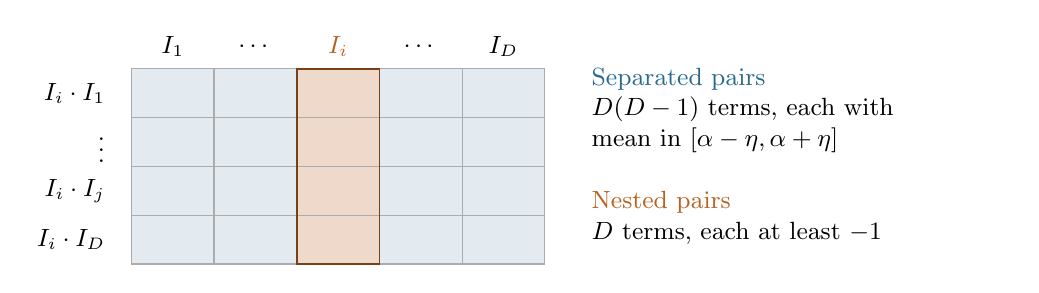
\begin{tikzpicture}[x=1.05cm,y=0.62cm,font=\small]
  \foreach \x in {0,1,2,3,4} {
    \foreach \y in {0,1,2,3} {
      \fill[parentblue!13] (\x,\y) rectangle +(1,1);
    }
  }
  \fill[childorange!24] (2,0) rectangle (3,4);
  \draw[gray!65,thin] (0,0) grid[xstep=1,ystep=1] (5,4);
  \draw[childorange!65!black,semithick] (2,0) rectangle (3,4);
  \node at (0.5,4.45) {$I_1$};
  \node at (1.5,4.45) {$\cdots$};
  \node[childorange] at (2.5,4.45) {$I_i$};
  \node at (3.5,4.45) {$\cdots$};
  \node at (4.5,4.45) {$I_D$};
  \node[anchor=east] at (-0.2,3.5) {$I_i\cdot I_1$};
  \node[anchor=east] at (-0.2,2.5) {$\vdots$};
  \node[anchor=east] at (-0.2,1.5) {$I_i\cdot I_j$};
  \node[anchor=east] at (-0.2,0.5) {$I_i\cdot I_D$};
  \node[anchor=west,align=left,text width=5.2cm] at (5.45,3.15)
    {\textcolor{parentblue}{Separated pairs}\\
     \(D(D-1)\) terms, each with\\
     mean in \([\alpha-\eta,\alpha+\eta]\)};
  \node[anchor=west,align=left,text width=5.2cm] at (5.45,0.95)
    {\textcolor{childorange}{Nested pairs}\\
     \(D\) terms, each at least \(-1\)};
\end{tikzpicture}
\caption{For fixed \(i\), the \((j,k)\) entry is
\(\ip{X_{I_i\cdot I_j}}{X_{I_k}}\). Rows index the children of
\(I_i\) and columns index all parents; the grid is schematic.
Only column \(i\) contains nested pairs, a fraction \(1/D\) of the
\(D^2\) terms.}
\label{fig:mixed-pairs}
\end{figure}

\emph{Step 5 (variance estimate).} Since
\(\norm{z_i-m}^2=\norm{z_i}^2+\norm m^2-2\ip{z_i}{m}\) and \(\EA\) is
linear, \eqref{avg:parent-bound}--\eqref{avg:mixed-bound} give
\begin{align}
  \EA\norm{z_i-m}^2
  &\le 2\Bigl[\Bigl(1-\frac1D\Bigr)(\alpha+\eta)+\frac1D\Bigr]
      -2\Bigl[\Bigl(1-\frac1D\Bigr)(\alpha-\eta)-\frac1D\Bigr]\notag\\
  &=\frac4D+4\Bigl(1-\frac1D\Bigr)\eta
    \qquad(1\le i\le D).
    \label{avg:variance}
\end{align}
The terms in \(\alpha\) cancel, so no assumption on the sign or size of
\(\alpha\) is needed.

\emph{Step 6 (conclusion).} Average \eqref{avg:displacement} over
\(g\in A\) and apply \eqref{avg:variance} to each of the \(D\) summands:
\[
  \delta^2
  \le\frac{L^2}{D}\sum_{i=1}^D\EA\norm{z_i-m}^2
  \le L^2\Bigl(\frac4D+4\Bigl(1-\frac1D\Bigr)\eta\Bigr).
\]
Divide by \(L^2\), subtract \(4/D\), and divide by \(4(1-1/D)>0\)
(recall \(D\ge2\)):
\[
  \eta\ge\frac{\delta^2/L^2-4/D}{4(1-1/D)} .
\]
The numerator is positive because \(D>4L^2/\delta^2\) by
\eqref{color:parameters}. The bound does not depend on \(A\).
\end{proof}

\begin{proof}[Proof of Theorem~\ref{thm:main}]
Let \(c_0>0\) be the right-hand side of \eqref{avg:boundary-bound}.
Suppose \(F\) were amenable. The F\o lner criterion \eqref{eq:folner},
applied to the finite set \(S\) and \(\varepsilon=c_0\), would give a
nonempty finite \(A\subset F\) with \(|hA\triangle A|/|A|<c_0\) for all
\(h\in S\). This contradicts Proposition~\ref{avg:boundary}.
\end{proof}

\section{Consequences}\label{sec:consequences}

The source records two corollaries. Each is obtained by quoting a theorem
from a companion paper. The source does not reproduce the statements of
those theorems, so all that can be checked here is that \(F\) satisfies
the hypotheses the source names; the companion theorems themselves are
not verified in this document. Neither is used in the proof of
Theorem~\ref{thm:main}.

\emph{Notation changed in this section only:} the Hilbert space is
\(\mathcal K\) and the conjugating operator \(V\) (source: \(H\), \(S\));
the generating set is \(\Sigma\), the Cayley graph
\(\mathrm{Cay}(F,\Sigma)\), the percolation parameter \(\mathsf p\), the
connection kernel \(\Lambda_{\mathsf p}\), and the edge labels
\(\zeta_e\) (source: \(S\), \(G_S\), \(p\), \(T_p\), \(U_e\)).

\subsection{Uniformly bounded representations}

\begin{corollary}[source Corollary~3.1]\label{cor:nonunitarizable}
For every \(\varepsilon>0\), there are a separable complex Hilbert space
\(\mathcal K\) and a representation
\(\pi:F\to\mathrm{GL}(\mathcal K)\) such that
\(\sup_{g\in F}\norm{\pi(g)}\le1+\varepsilon\), but no bounded invertible
operator \(V\) on \(\mathcal K\) makes every \(V\pi(g)V^{-1}\) unitary.
\end{corollary}

\begin{proof}
\(F\) is countable: an element is determined by a finite list of dyadic
breakpoints and integer slope exponents. \(F\) is nonamenable by
Theorem~\ref{thm:main}. The source then concludes from the companion
unitarizability theorem \cite[Theorem~1.1]{OpenAIUnitarizability2026},
which it applies to countable nonamenable groups.

\unverified{This conclusion rests entirely on the cited companion theorem,
whose statement and hypotheses the source does not reproduce. As used
here, it would give a non-unitarizable uniformly bounded representation
with bound \(1+\varepsilon\) for \emph{every} countable nonamenable group
(a Dixmier-type statement). That cannot be checked from this manuscript,
and it goes beyond what is known to be established in that generality.
The corollary is not used in the proof of Theorem~\ref{thm:main}.}
\end{proof}

\subsection{Percolation on Cayley graphs}

For a finite symmetric generating set
\(\Sigma\subset F\setminus\{\id\}\), let \(\mathrm{Cay}(F,\Sigma)\) be the
simple undirected Cayley graph with edges \(\{x,xs\}\), \(s\in\Sigma\).
In Bernoulli bond percolation each edge is independently open with
probability \(\mathsf p\). Write \(\mathsf p_c\) for the threshold for
existence of an infinite open cluster and \(\mathsf p_u\) for the
threshold for almost-sure uniqueness of the infinite open cluster. The
connection kernel
\(\Lambda_{\mathsf p}(x,y)=\mathbb P_{\mathsf p}(x\leftrightarrow y)\)
acts on counting-measure \(\ell^2(F)\), initially on finitely supported
functions by summation over \(y\); put
\(\mathsf p_{2\to2}=\sup\{\mathsf p\in[0,1]:
\Lambda_{\mathsf p}\text{ is bounded on }\ell^2(F)\}\).

\begin{corollary}[source Corollary~3.2]\label{cor:percolation}
For every such generating set \(\Sigma\),
\[
  \norm{\Lambda_{\mathsf p_c}}_{2\to2}<\infty,\qquad
  \mathsf p_c<\mathsf p_{2\to2}\le \mathsf p_u.
\]
For each fixed \(\mathsf p\in(\mathsf p_c,\mathsf p_u)\), there are almost
surely infinitely many infinite open clusters. Moreover, there are
deterministic \(\mathsf p_c<\mathsf p_1<\mathsf p_2<1\), depending on
\(\Sigma\), such that in the coupling with independent uniform \([0,1]\)
edge labels \(\zeta_e\), opening \(e\) when \(\zeta_e\le\mathsf p\), there
are almost surely infinitely many infinite open clusters simultaneously
for every \(\mathsf p\in[\mathsf p_1,\mathsf p_2]\).
\end{corollary}

\begin{proof}
The source applies the companion percolation result
\cite[Corollary~1.2]{OpenAIPercolation2026} to \(F\), which is
nonamenable by Theorem~\ref{thm:main}.

\unverified{This conclusion rests entirely on the cited companion result,
whose statement and hypotheses the source does not reproduce. As used
here, it would give \(\mathsf p_c<\mathsf p_{2\to2}\le\mathsf p_u\) and the
other stated conclusions for \emph{every} Cayley graph of a nonamenable
group. That cannot be checked from this manuscript, and it goes beyond
what is known to be established in that generality. The corollary is not
used in the proof of Theorem~\ref{thm:main}.}
\end{proof}

\appendix
\section{An explicit map with positive displacement}\label{app:auxiliary}

This appendix proves the Hilbert-space instance of the
Benyamini--Sternfeld theorem~\cite{BenyaminiSternfeld1983} directly, which
gives Lemma~\ref{lem:displacement} with \(\delta=1/2\). It is independent
of Sections~\ref{sec:dyadic}--\ref{sec:consequences}. The letters
\(a,b,c,d,e,q,r,s,t,u,v,M,U,G\) have the meanings defined \emph{here};
only \(H,B,f\) play the role they have in Lemma~\ref{lem:displacement}.
\emph{Renamings relative to the source's appendix:} the nearest-point
parameter is \(\tau(x)\) (source: \(t(x)\)), the argument of \(\sinc\) is
\(\omega\) (source: \(q\)), the quarter-turn of \(\R^2\) is \(\Pi\)
(source: \(J\)), and the Lipschitz constant of \(\gamma'\) is
\(K_\gamma\) (source: \(K\)).

Throughout, \(H=L^2([0,1];\R^2)\) with
\(\ip xy=\int_0^1x(w)\cdot y(w)\,dw\), and \(B\) is its closed unit ball.

\begin{proposition}[source Proposition~A.1]\label{aux:map}
There is a globally Lipschitz map \(f:B\to B\) such that
\[
  \norm{f(x)}=1,
  \qquad \norm{f(x)-x}\ge\frac12
  \quad(x\in B).
\]
\end{proposition}

\paragraph{Plan.} We construct a Lipschitz map \(G:B\to H\) with
\(\norm{G(x)}\ge\rho/4>0\) for all \(x\), and \(G(x)=x\) whenever
\(\norm x\ge1/2\). Then \(f(x)=-G(x)/\norm{G(x)}\) works. The map \(G\) is
the identity outside a thin tube \(U\) around a curve \(\gamma\) through
the origin. Inside the tube it replaces the curve point
\(\gamma(t)=a(t)v(t)\) by \(b(t)v(t)\) with \(b\le-1/8\).
Lemma~\ref{aux:tube} shows the tube has a well-behaved nearest-point
projection, although the curve has a bounded tail.
Lemma~\ref{aux:rotation} supplies rotations that keep the residual
\(x-\gamma(t)\) orthogonal to \(v(t)\), so it cannot cancel the new
coefficient.

One elementary fact is used twice.
\begin{equation}\label{aux:normalize}
  \Bigl\|\frac{y}{\norm y}-\frac{y'}{\norm{y'}}\Bigr\|
  \le\frac{2}{\kappa}\norm{y-y'}
  \qquad\text{if }\norm y,\norm{y'}\ge\kappa>0 .
\end{equation}
Indeed the left side is at most
\(\norm{y-y'}/\norm y+\norm{y'}\,\bigl|\norm{y}^{-1}-\norm{y'}^{-1}\bigr|
=\norm{y-y'}/\norm y+\bigl|\norm{y'}-\norm y\bigr|/\norm y\).

\subsection{The curve}

Define functions on \(\R\) by
\[
 a(t)=
 \begin{cases}
 t/8,&t\le2,\\
 5/16-(3-t)^2/16,&2<t<3,\\
 5/16,&t\ge3,
 \end{cases}
 \qquad
 \theta(t)=
 \begin{cases}
 0,&t\le1,\\
 (t-1)^2/2,&1<t<2,\\
 t-3/2,&t\ge2.
 \end{cases}
\]
\begin{center}
\begin{tabular}{@{}lcccc@{}}
\toprule
range of \(t\) & \(a(t)\) & \(a'(t)\) & \(\theta(t)\) & \(\theta'(t)\)\\
\midrule
\(t\le1\) & \(t/8\) & \(1/8\) & \(0\) & \(0\)\\
\(1\le t\le2\) & \(t/8\) & \(1/8\) & \((t-1)^2/2\) & \(t-1\)\\
\(2\le t\le3\) & \(5/16-(3-t)^2/16\) & \((3-t)/8\) & \(t-3/2\) & \(1\)\\
\(t\ge3\) & \(5/16\) & \(0\) & \(t-3/2\) & \(1\)\\
\bottomrule
\end{tabular}
\end{center}
At the junctions the table's entries agree
(\(a(2)=1/4\), \(a'(2)=1/8\), \(a(3)=5/16\), \(a'(3)=0\);
\(\theta(1)=\theta'(1)=0\), \(\theta(2)=1/2\), \(\theta'(2)=1\)). Hence:
\begin{enumerate}[label=(F\arabic*)]
\item \(a,\theta\) are \(C^1\); \(a'\) and \(\theta'\) are continuous and
piecewise affine, hence Lipschitz (constants \(1/8\) and \(1\)).
\item \(0\le a'\le1/8\) and \(0\le\theta'\le1\); \(\theta'=0\) on
\((-\infty,1]\).
\item \(a\) is nondecreasing, \(a\le5/16\) everywhere, \(a(t)\ge1/8\) for
\(t\ge1\), \(a(t)\ge1/4\) for \(t\ge2\), and \(a(t)=5/16\) for \(t\ge3\).
\item \(\theta=0\) on \((-\infty,1]\), \(\theta\) is strictly increasing
on \([1,\infty)\), \(\theta(t)\to\infty\), and
\(\theta(t)-\theta(s)=t-s\) for \(s,t\ge2\).
\end{enumerate}
For \(t\in\R\) and \(w\in[0,1]\) put
\[
 v(t)(w)=(\cos(\theta(t)w),\sin(\theta(t)w)),
 \qquad \gamma(t)=a(t)v(t)\in H .
\]
\begin{enumerate}[label=(F\arabic*),resume]
\item \(\norm{v(t)}=1\), since \(|v(t)(w)|=1\) for all \(w\). Pointwise
\(|v(t)(w)-v(s)(w)|\le|\theta(t)-\theta(s)|\,w\le|t-s|\), so
\(\norm{v(t)-v(s)}\le|t-s|\).
\end{enumerate}
Thus \(\gamma(0)=0\) and \(\norm{\gamma(t)}=|a(t)|\). For \(t\le1\),
\(v(t)\) is the constant function \((1,0)\) and \(\gamma(t)=(t/8)v(1)\)
is a straight line. For \(t\ge1\), \(\norm{\gamma(t)}\le5/16\).

\subsection{The tube around the curve}

\begin{lemma}[source Lemma~A.2]\label{aux:tube}
The curve \(\gamma\) is injective, has a bounded Lipschitz derivative, and
\[
 c:=\inf_{t\in\R}\norm{\gamma'(t)}=\frac18.
\]
Its unit tangent \(u(t)=\gamma'(t)/\norm{\gamma'(t)}\) is Lipschitz,
\(\ip{u(t)}{v(t)}\ge0\), and \(u(t)=v(t)\) for \(t\le1\).
There is a radius \(0<\rho<1/32\) such that every point in
\[
 U=\{x\in H:\dist(x,\gamma(\R))<\rho\}
\]
has a unique nearest point \(\gamma(\tau(x))\) on the curve. Writing
\(e(x)=x-\gamma(\tau(x))\), we have \(e(x)\perp u(\tau(x))\), and
\begin{equation}\label{aux:parameter}
 |\tau(x)-\tau(y)|\le16\norm{x-y}
 \quad\text{if }x,y\in U\text{ and }\norm{x-y}<\rho.
\end{equation}
\end{lemma}
\noindent\emph{Used in:} the definition of \(G\) and all three steps of
the proof of Proposition~\ref{aux:map}.

\begin{proof}
Let \(\Pi(\xi_1,\xi_2)=(-\xi_2,\xi_1)\) be the quarter-turn of \(\R^2\).

\emph{Step 1 (derivative, speed).} For fixed \(w\), the \(\R^2\)-valued
function \(t\mapsto\gamma(t)(w)\) is \(C^1\) by (F1), with derivative
\[
 \Gamma(t)(w):=a'(t)\,v(t)(w)+a(t)\theta'(t)\,w\,\Pi v(t)(w).
\]
\emph{Claim: there is \(K_\gamma<\infty\) with
\(|\Gamma(t)(w)-\Gamma(s)(w)|\le K_\gamma|t-s|\) for all
\(s,t\in\R\), \(w\in[0,1]\).} A product of bounded Lipschitz functions is
Lipschitz, so it suffices that the four factors are bounded and Lipschitz
in \(t\), uniformly in \(w\): \(a'\) by (F1), (F2); \(v(t)(w)\) and
\(w\,\Pi v(t)(w)\) by (F5); and \(a\theta'\) because it vanishes on
\((-\infty,1]\), while on \([1,\infty)\) both \(a\in[1/8,5/16]\) and
\(\theta'\in[0,1]\) are bounded and Lipschitz. (This is where the
unboundedness of \(a\) as \(t\to-\infty\) is harmless.)

Integrating in \(t\) for fixed \(w\),
\(\gamma(t)(w)-\gamma(s)(w)-(t-s)\Gamma(s)(w)
=\int_s^t(\Gamma(\lambda)(w)-\Gamma(s)(w))\,d\lambda\) has absolute value
at most \(\tfrac12K_\gamma|t-s|^2\) for every \(w\). Taking the \(L^2\)
norm in \(w\),
\begin{equation}\label{aux:taylor}
 \norm{\gamma(t)-\gamma(s)-(t-s)\Gamma(s)}
 \le\frac{K_\gamma}{2}|t-s|^2 .
\end{equation}
So \(\gamma\) is differentiable as an \(H\)-valued map with
\(\gamma'=\Gamma\), and \(\norm{\gamma'(t)-\gamma'(s)}\le K_\gamma|t-s|\).
Since \(v(t)(w)\perp\Pi v(t)(w)\) are unit vectors of \(\R^2\),
\[
 \norm{\gamma'(t)}^2=a'(t)^2+a(t)^2\theta'(t)^2\int_0^1w^2\,dw
 =a'(t)^2+\frac{a(t)^2\theta'(t)^2}{3}.
\]
This is bounded; put \(M=\sup_t\norm{\gamma'(t)}<\infty\). For \(t\le2\)
the first term is \(1/64\), with equality \(\norm{\gamma'(t)}=1/8\) when
\(t\le1\). For \(t\ge2\), \(a\ge1/4\) and \(\theta'=1\) give at least
\(1/48>1/64\). Hence \(c=1/8\).

\emph{Step 2 (unit tangent).} By \eqref{aux:normalize} with \(\kappa=c\),
\(u\) is Lipschitz; put \(K_u=\Lip(u)\). Since
\(\ip{\Pi v(t)(w)}{v(t)(w)}=0\) pointwise,
\(\ip{\gamma'(t)}{v(t)}=a'(t)\), so
\(\ip{u(t)}{v(t)}=a'(t)/\norm{\gamma'(t)}\ge0\). For \(t\le1\),
\(\gamma'(t)=\tfrac18v(t)\), so \(u(t)=v(t)\).

\emph{Step 3 (injectivity).} With \(\sinc(\omega)=\sin(\omega)/\omega\)
for \(\omega\ne0\) and \(\sinc(0)=1\),
\[
 \ip{v(s)}{v(t)}=\int_0^1\cos\bigl((\theta(t)-\theta(s))w\bigr)\,dw
 =\sinc(\theta(t)-\theta(s)),
\]
and therefore
\begin{equation}\label{aux:distance}
 \norm{\gamma(t)-\gamma(s)}^2
 =a(t)^2+a(s)^2-2a(t)a(s)\sinc(\theta(t)-\theta(s)).
\end{equation}
Since \(|\sinc(\omega)|<1\) for \(\omega\ne0\), unit vectors \(v(s),v(t)\)
with \(\theta(s)\ne\theta(t)\) are linearly independent (strict
Cauchy--Schwarz). Let \(s<t\). If \(t\le1\), then
\(\gamma(t)-\gamma(s)=\tfrac{t-s}{8}v(1)\ne0\). If \(t>1\), then
\(\theta(t)>\theta(s)\) by (F4), so \(v(s),v(t)\) are independent, and
\(a(t)\ge1/8>0\) by (F3); hence \(a(t)v(t)-a(s)v(s)\ne0\).

\emph{Step 4 (uniform separation).} \emph{Claim:}
\begin{equation}\label{aux:separation}
 \sigma(d):=\inf_{|t-s|\ge d}\norm{\gamma(t)-\gamma(s)}>0
 \qquad(d>0).
\end{equation}
Suppose not. Choose \(s_n<t_n\) with \(t_n-s_n\ge d\) and
\(\norm{\gamma(t_n)-\gamma(s_n)}\to0\), and pass to a subsequence with
\(s_n\to s_*\), \(t_n\to t_*\) in \([-\infty,+\infty]\), \(s_*\le t_*\).
\begin{itemize}
\item \emph{Both finite.} Then \(t_*-s_*\ge d\) and, by continuity,
\(\gamma(t_*)=\gamma(s_*)\), contradicting Step~3.
\item \emph{\(s_*=t_*=-\infty\).} Eventually \(s_n<t_n\le1\), and the
distance is \((t_n-s_n)/8\ge d/8\).
\item \emph{\(s_*=-\infty<t_*\).} Then
\(\norm{\gamma(s_n)}=|s_n|/8\to\infty\), while \(t_n\ge t_0\) for some
\(t_0\) and hence
\(\norm{\gamma(t_n)}=|a(t_n)|\le\max\{|a(t_0)|,5/16\}\) by (F3). The
distance tends to infinity.
\item \emph{\(s_*\) finite, \(t_*=+\infty\).} Then
\(\theta(t_n)-\theta(s_n)\to\infty\), so the \(\sinc\) term in
\eqref{aux:distance} tends to \(0\), and the squared distance tends to
\(a(s_*)^2+(5/16)^2>0\).
\item \emph{\(s_*=t_*=+\infty\).} Eventually \(s_n,t_n\ge3\), so
\(a=5/16\) and \(\theta(t_n)-\theta(s_n)=t_n-s_n\ge d\), and by
\eqref{aux:distance}
\[
 \norm{\gamma(t_n)-\gamma(s_n)}^2
 =2(5/16)^2\bigl(1-\sinc(t_n-s_n)\bigr)
 \ge2(5/16)^2\bigl(1-\sup_{\omega\ge d}\sinc(\omega)\bigr)>0 .
\]
The supremum is \(<1\): \(\sinc(\omega)\le1/\omega\le1/2\) for
\(\omega\ge2\), and on the compact interval \([d,\max\{d,2\}]\) the
continuous function \(\sinc\) is everywhere \(<1\).
\end{itemize}
Each case contradicts \(\norm{\gamma(t_n)-\gamma(s_n)}\to0\).

\emph{Step 5 (tangent estimate; choice of \(d\) and \(\rho\)).} Choose
\(d>0\) with \(K_\gamma d\le c/2\). For \(|t-s|\le d\), pair
\eqref{aux:taylor} with \(u(s)\) and use
\(\ip{\gamma'(s)}{u(s)}=\norm{\gamma'(s)}\ge c\):
\begin{equation}\label{aux:tangent}
 |\ip{\gamma(t)-\gamma(s)}{u(s)}|
 \ge c|t-s|-\frac{K_\gamma d}{2}|t-s|
 \ge\frac{3c}{4}|t-s|
 \qquad(|t-s|\le d).
\end{equation}
Choose \(\rho>0\) so that
\begin{equation}\label{aux:radius}
 \rho<\frac1{32},\qquad 4\rho<\sigma(d),\qquad \rho K_u<\frac c4.
\end{equation}

\emph{Step 6 (a nearest point exists and \(e\perp u\)).} Let \(x\in U\)
and let \(\gamma(t_n)\) be a minimizing sequence for
\(\dist(x,\gamma(\R))<\rho\). For \(n\ge n_1\),
\(\norm{x-\gamma(t_n)}<2\rho\), so for \(n,n'\ge n_1\),
\(\norm{\gamma(t_n)-\gamma(t_{n'})}<4\rho<\sigma(d)\), which by the
definition of \(\sigma(d)\) forces \(|t_n-t_{n'}|<d\). So
\(t_n\in[t_{n_1}-d,t_{n_1}+d]\) for \(n\ge n_1\); a convergent
subsequence has a limit \(t_*\), and by continuity \(\gamma(t_*)\)
attains the minimum. At any minimizing parameter \(t\), the derivative
\(-2\ip{x-\gamma(t)}{\gamma'(t)}\) of \(\norm{x-\gamma(t)}^2\) vanishes,
so \((x-\gamma(t))\perp u(t)\).

\emph{Step 7 (parameter estimate and uniqueness).} Let \(x,y\in U\) with
\(\norm{x-y}<\rho\), let \(t,s\) be \emph{any} minimizing parameters for
\(x,y\), and write \(x=\gamma(t)+e_t\), \(y=\gamma(s)+e_s\), with
\(\norm{e_t},\norm{e_s}<\rho\), \(e_t\perp u(t)\), \(e_s\perp u(s)\).
Then \(\norm{\gamma(t)-\gamma(s)}<3\rho<\sigma(d)\), so \(|t-s|<d\).
Since \(\ip{e_s}{u(s)}=0\) and
\(\ip{e_t}{u(s)}=\ip{e_t}{u(s)-u(t)}\),
\begin{align*}
 \norm{x-y}\ge|\ip{x-y}{u(s)}|
 &\ge |\ip{\gamma(t)-\gamma(s)}{u(s)}|
       -|\ip{e_t}{u(s)-u(t)}|\\
 &\ge\Bigl(\frac{3c}{4}-\rho K_u\Bigr)|t-s|
 \ge\frac c2|t-s|=\frac{1}{16}|t-s| ,
\end{align*}
by \eqref{aux:tangent} and \eqref{aux:radius}. Taking \(y=x\) shows the
minimizing parameter is unique; call it \(\tau(x)\). The same inequality
is \eqref{aux:parameter}.
\end{proof}

\subsection{Rotating the tangent onto the radial direction}

\begin{lemma}[source Lemma~A.3]\label{aux:rotation}
There is a family of orthogonal operators \(R_t:H\to H\), Lipschitz in
operator norm, such that \(R_tu(t)=v(t)\) and \(R_t\) is the identity for
\(t\le1\).
\end{lemma}
\noindent\emph{Used in:} the definition of \(G\); the property
\(R_tu(t)=v(t)\) gives \(R_te\perp v(t)\) for \(e\perp u(t)\).

\begin{proof}
Suppress \(t\) and put \(\kappa=\ip uv\ge0\) (Lemma~\ref{aux:tube}).
Define
\[
 Ah=v\ip{u}{h}-u\ip{v}{h},
 \qquad R=\mathrm{Id}+A+\frac{A^2}{1+\kappa}.
\]

\emph{Case \(u,v\) linearly independent.} \(A\) is skew-adjoint:
\(\ip{Ah}{k}=\ip vk\ip uh-\ip uk\ip vh=-\ip h{Ak}\). It vanishes on
\(\{u,v\}^\perp\) and preserves \(\mathrm{span}\{u,v\}\), where
\(Au=v-\kappa u\) and \(Av=\kappa v-u\). Hence
\(A^2u=\kappa v-u-\kappa(v-\kappa u)=-(1-\kappa^2)u\) and
\(A^2v=\kappa(\kappa v-u)-(v-\kappa u)=-(1-\kappa^2)v\). So on the span,
\(R=\mathrm{Id}+A-(1-\kappa)\mathrm{Id}=\kappa\,\mathrm{Id}+A\). There
\(Ru=\kappa u+v-\kappa u=v\), and
\((\kappa\,\mathrm{Id}+A)^*(\kappa\,\mathrm{Id}+A)
=\kappa^2\mathrm{Id}-A^2=\mathrm{Id}\), so \(R\) is orthogonal on the
span. On the orthogonal complement \(R=\mathrm{Id}\). So \(R\) is
orthogonal on \(H\).

\emph{Case \(u,v\) dependent.} Unit vectors with \(\ip uv\ge0\) that are
dependent are equal, so \(A=0\) and \(R=\mathrm{Id}\), and \(Ru=v\).

\emph{Lipschitz dependence.} \(u\) and \(v\) are bounded and Lipschitz in
\(t\) (Lemma~\ref{aux:tube}, (F5)), hence so are \(A_t\) in operator norm
(\(\norm{A_t-A_s}\le2\norm{u(t)-u(s)}+2\norm{v(t)-v(s)}\),
\(\norm{A_t}\le2\)), \(A_t^2\), \(\kappa\), and \(1/(1+\kappa)\) (as
\(1+\kappa\ge1\)). So \(t\mapsto R_t\) is Lipschitz, uniformly across
both cases. For \(t\le1\), \(u(t)=v(t)\) and \(R_t=\mathrm{Id}\).
\end{proof}

\subsection{Proof of Proposition~\ref{aux:map}}

\begin{proof}
Fix \(\rho\), \(U\), \(\tau\), \(e\) from Lemma~\ref{aux:tube}, \(R_t\)
from Lemma~\ref{aux:rotation}, and \(M=\sup_t\norm{\gamma'(t)}\).

\emph{Step 0 (definition of \(G\)).} Set
\[
 b(t)=\min\{a(t),-1/8\},\qquad
 q(t)=b(t)-a(t)=-\max\{a(t)+1/8,0\}.
\]
Then \(|q(t)|\le5/16+1/8=7/16\) by (F3), \(\Lip(q)\le\Lip(a)=1/8\), and
\(q(t)=0\) when \(a(t)\le-1/8\). Let
\(\beta,\chi:[0,\infty)\to[0,1]\) be
\[
 \beta(r)=
 \begin{cases}
 1,&r\le\rho/4,\\
 2-4r/\rho,&\rho/4<r<\rho/2,\\
 0,&r\ge\rho/2,
 \end{cases}
 \qquad
 \chi(r)=
 \begin{cases}
 1,&r\le\rho/2,\\
 2-2r/\rho,&\rho/2<r<\rho,\\
 0,&r\ge\rho.
 \end{cases}
\]
They are continuous with Lipschitz constants \(4/\rho\) and \(2/\rho\),
and
\begin{equation}\label{aux:cutoffs}
 \beta(r)\le\chi(r)\le\frac{2(\rho-r)}{\rho}\qquad(0\le r<\rho):
\end{equation}
for \(r\ge\rho/2\) the second inequality is an equality, and for
\(r\le\rho/2\) its right side is \(\ge1\).
Define \(G:B\to H\) by \(G(x)=x\) for \(x\notin U\), and for
\(x\in B\cap U\), with \(t=\tau(x)\), \(e=e(x)=x-\gamma(t)\),
\(r=\norm e=\dist(x,\gamma(\R))<\rho\),
\begin{equation}\label{aux:G}
 \begin{split}
 G(x)&=\gamma(t)+\beta(r)q(t)v(t)
       +\bigl((1-\chi(r))\mathrm{Id}+\chi(r)R_t\bigr)e\\
 &=x+\beta(r)q(t)v(t)+\chi(r)(R_t-\mathrm{Id})e .
 \end{split}
\end{equation}
The two lines agree because \(x=\gamma(t)+e\).

\emph{Step 1 (\(G\) is globally Lipschitz on \(B\)).} Let \(x,y\in B\).

\emph{(1a) \(x,y\in U\), \(\norm{x-y}<\rho\).} By \eqref{aux:parameter},
\(|\tau(x)-\tau(y)|\le16\norm{x-y}\). Hence
\[
 \norm{e(x)-e(y)}\le\norm{x-y}+\norm{\gamma(\tau(x))-\gamma(\tau(y))}
 \le(1+16M)\norm{x-y},
\]
and \(r(x)=\dist(x,\gamma(\R))\) is \(1\)-Lipschitz. So each factor in
the second line of \eqref{aux:G}, namely \(\beta(r)\), \(q(t)\), \(v(t)\),
\(\chi(r)\), \(R_t-\mathrm{Id}\), \(e\), is Lipschitz on such pairs with
a constant independent of the pair. Each is bounded: \(\beta,\chi\le1\),
\(|q|\le7/16\), \(\norm v=1\), \(\norm{R_t-\mathrm{Id}}\le2\),
\(\norm e<\rho\). Products of bounded Lipschitz factors are Lipschitz, so
there is one constant \(L_1\) with
\(\norm{G(x)-G(y)}\le L_1\norm{x-y}\) for all such pairs.

\emph{(1b) \(\norm{x-y}\ge\rho\).} For every \(x\in B\),
\(\norm{G(x)}\le1+7/16+2\rho<3/2\) (by \eqref{aux:G} inside \(U\);
trivially outside). So
\(\norm{G(x)-G(y)}<3\le(3/\rho)\norm{x-y}\).

\emph{(1c) \(x\in U\), \(y\notin U\), \(\norm{x-y}<\rho\).} By
\eqref{aux:G}, \eqref{aux:cutoffs}, and \(r<\rho\),
\[
 \norm{G(x)-x}\le\beta(r)\cdot\frac7{16}+\chi(r)\cdot2r
 \le\frac{2(\rho-r)}{\rho}\Bigl(\frac7{16}+2\rho\Bigr)
 =\Bigl(\frac{7}{8\rho}+4\Bigr)(\rho-r).
\]
Since distance to the curve is \(1\)-Lipschitz and
\(\dist(y,\gamma(\R))\ge\rho\), \(\rho-r\le\norm{x-y}\). With \(G(y)=y\),
\(\norm{G(x)-G(y)}\le\bigl(\tfrac7{8\rho}+5\bigr)\norm{x-y}\).

\emph{(1d) \(x,y\notin U\).} \(G\) is the identity. These four cases
cover all pairs.

\emph{Step 2 (\(G\) is bounded away from zero).} \emph{Claim:}
\begin{equation}\label{aux:nonzero}
 \norm{G(x)}\ge\rho/4\qquad(x\in B).
\end{equation}
\emph{Outside \(U\):} since \(0=\gamma(0)\),
\(\norm{G(x)}=\norm x\ge\dist(x,\gamma(\R))\ge\rho\).

\emph{Inside \(U\), \(r\le\rho/2\):} here \(\chi(r)=1\), so by the first
line of \eqref{aux:G},
\(G(x)=\bigl(a(t)+\beta(r)q(t)\bigr)v(t)+R_te\). Since \(e\perp u(t)\),
\(R_t\) is orthogonal and \(R_tu(t)=v(t)\), we get
\(\ip{R_te}{v(t)}=\ip e{u(t)}=0\) and \(\norm{R_te}=r\). So
\(\norm{G(x)}^2=(a+\beta q)^2+r^2\). If \(r\le\rho/4\), then \(\beta=1\),
\(a+q=b\le-1/8\), and \(\norm{G(x)}\ge1/8>\rho/4\). If
\(\rho/4\le r\le\rho/2\), then \(\norm{G(x)}\ge r\ge\rho/4\).

\emph{Inside \(U\), \(\rho/2\le r<\rho\):} here \(\beta(r)=0\), so
\(G(x)=\gamma(t)+\bigl((1-\chi)\mathrm{Id}+\chi R_t\bigr)e\), and the
last term has norm at most \((1-\chi)r+\chi r=r<\rho\). If \(t>1\), then
\(\norm{\gamma(t)}=a(t)\ge1/8\) by (F3), so
\(\norm{G(x)}\ge1/8-\rho>\rho/4\) (as \(\rho<1/32\)). If \(t\le1\), then
\(R_t=\mathrm{Id}\), so \(G(x)=\gamma(t)+e=a(t)v(t)+e\) with
\(e\perp u(t)=v(t)\), and \(\norm{G(x)}\ge r\ge\rho/2\).

\emph{Step 3 (\(G(x)=x\) whenever \(\norm x\ge1/2\)).} Outside \(U\) this
is the definition. Inside \(U\),
\[
 |a(t)|=\norm{\gamma(t)}\ge\norm x-r>\frac12-\rho>\frac12-\frac1{32}
 >\frac5{16}.
\]
Since \(a\le5/16\) everywhere, this forces \(a(t)<-5/16<-1/8\), hence
\(t\le1\). So \(q(t)=0\) and \(R_t=\mathrm{Id}\), and the second line of
\eqref{aux:G} gives \(G(x)=x\).

\emph{Step 4 (the map \(f\)).} Define
\[
 f(x)=-\frac{G(x)}{\norm{G(x)}}\qquad(x\in B).
\]
By \eqref{aux:nonzero} this is well defined with \(\norm{f(x)}=1\), so
\(f:B\to B\). By \eqref{aux:normalize} with \(\kappa=\rho/4\),
normalization is Lipschitz with constant at most \(8/\rho\) on the range
of \(G\), so \(f\) is globally Lipschitz by Step~1. If \(\norm x<1/2\),
then \(\norm{f(x)-x}\ge\norm{f(x)}-\norm x=1-\norm x>1/2\). If
\(\norm x\ge1/2\), then \(G(x)=x\) by Step~3, so \(f(x)=-x/\norm x\) and
\(\norm{f(x)-x}=1+\norm x\ge3/2\).
\end{proof}

\section*{Verification checklist}
\addcontentsline{toc}{section}{Verification checklist}

The load-bearing steps, in the order a sceptical reader should check them.
\begin{enumerate}
\item \textbf{Covariance and its use} (Lemma~\ref{dyad:covariance};
Step~1 of Proposition~\ref{avg:boundary}). Check that
\(X_I(g)=X_{I_1}(hg)\) and \(X_J(g)=X_{I_2}(hg)\) hold for the \emph{same}
\(h=h_{I,J}\) and the \emph{same} level \(n\), and that both \(g\) and
\(hg\) are admissible (Step~0: \(n\) is chosen for \(A\cup SA\)).
\item \textbf{Order of quantifiers.} \(S\) is fixed before \(A\)
(Section~\ref{sec:boundary}); only \(n\) depends on \(A\). The lower bound
\eqref{avg:boundary-bound} does not involve \(n\) or \(A\).
\item \textbf{Recursion identity} \(X_{I_i}=f(z_i)\) (Step~2), which
needs \((T_I)_J=T_{I\cdot J}\) (Lemma~\ref{dyad:calculus}(c)) and
admissibility for all children; and well-foundedness of the coloring
(Lemma~\ref{color:welldefined}).
\item \textbf{Bookkeeping of pairs} (Lemma~\ref{color:family}(b);
Step~4): exactly \(D(D-1)\) separated and \(D\) exceptional terms in each
of the three expansions, and the cancellation of \(\alpha\) in
\eqref{avg:variance}.
\item \textbf{Translation inequality matches the F\o lner criterion}
(Lemma~\ref{lem:finite-translation} and \eqref{eq:folner}): both concern
left translation \(A\mapsto hA\).
\item \textbf{Transport lemma} (Lemma~\ref{dyad:transport}), including
the flagged Step~3: the source equalizes only the total number of gap
cells; the argument needs equal counts in each gap.
\item \textbf{Final arithmetic} (Step~6) and the role of
\(D>4L^2/\delta^2\) \eqref{color:parameters}.
\item \textbf{Existence of \(f\)} (Lemma~\ref{lem:displacement}). If
relying on the appendix rather than the citation, check: uniform
separation \eqref{aux:separation} (five cases, Step~4 of
Lemma~\ref{aux:tube}); the parameter estimate \eqref{aux:parameter}
(Step~7); and the three cases of \(\norm{G}\ge\rho/4\) (Step~2 of the
proof of Proposition~\ref{aux:map}).
\item \textbf{Scope.} Corollaries~\ref{cor:nonunitarizable}
and~\ref{cor:percolation} rest on companion theorems that are quoted, not
proved or checked here.
\end{enumerate}

\bibliographystyle{plain}
\bibliography{sources}
\end{document}
